% 2008 年山东卷理科第 22 题：抛物线 x²=2py（p>0），M 为直线 y=-2p 上一点，
%   过 M 作抛物线两条切线，切点为 A、B。
% 来源 PDF：gaokaomath-src/普通高考/2008/2008山东理.pdf
% SHA-256：b4666951a0c2475fab098b837a343c7352003964f7811cedb1bdd610503e6e3b
% 原页：2008山东理.pdf 第 2 页（A3 三栏）第 3 栏，书页码 472。
% 重绘依据：取 p=1 画示意图：M(0,-2)，切点 A(-2,2)、B(2,2)，连 MA、MB 与弦 AB。
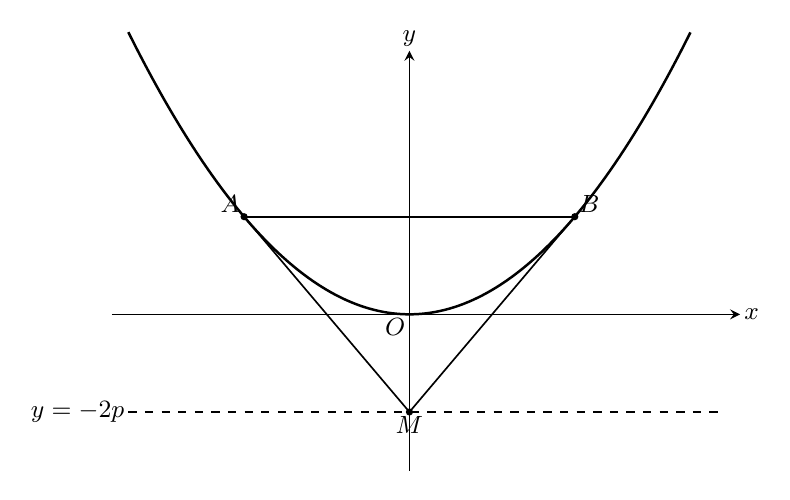
\begin{tikzpicture}[x=1.05cm, y=0.62cm, semithick, font=\small,
  every node/.style={inner sep=1.2pt}]
  \draw[->,>=stealth] (-3.6,0) -- (4.0,0) node[right] {$x$};
  \draw[->,>=stealth] (0,-3.2) -- (0,5.4) node[above] {$y$};
  \node[below left] at (0,0) {$O$};

  % 抛物线 y = x^2/2
  \draw[line width=0.9pt, domain=-3.4:3.4, samples=120] plot (\x, {\x*\x/2});

  % 直线 y = -2p
  \draw[dashed] (-3.4,-2) -- (3.8,-2);
  \node[left] at (-3.4,-2) {$y=-2p$};

  % 切点与切线
  \coordinate (A) at (-2,2);
  \coordinate (B) at (2,2);
  \coordinate (M) at (0,-2);
  \draw (M) -- (A);
  \draw (M) -- (B);
  \draw (A) -- (B);

  \fill (A) circle (1.3pt) node[above left] {$A$};
  \fill (B) circle (1.3pt) node[above right] {$B$};
  \fill (M) circle (1.3pt) node[below] {$M$};
\end{tikzpicture}
